\chapter{Introduction}
\section{Overview}
The objective of this thesis is twofold: Primarily this study focuses on varying fabrication methods using rapid prototyping (3-D printing) including changes in extrusion/fabrication orientation, fill percentage, and material in order to create the strongest structures with minimal waste possible. Secondarily, the aim was to provide a model to predict the behavior of structures fabricated using Fused Deposition Modeling under the various parameters tested. Beam specimens were designed in Solidworks and tested using a custom fixture designed and built for the purpose. All of the tensile test specimens were also designed using Solidworks and were intended to be tested according to the guidelines set forth in the ASME Standard Test Method for Tensile Properties of Plastics. \par
	In addition to the varied fabrication factors listed above the rapid prototyping was done using two different materials commonly found in the industry: PLA and ABS plastics. After an optimal method was discovered in fabricating both the PLA and ABS tensile test specimens, more complex structures were created and evaluated using both materials. The next step after completing the initial tensile testing was to create an I-Beam and predict the displacement based on the bending strength of the square and rectangular specimens. Finally, tensile test specimens were intended to be created and tested according to ASTM D638 for type I specimens \citep{ASTMNorma2004}. All test specimens used in the study were printed using Ultimaker 2 3D printer units, pictured in figure \ref{fig:Printer_Clean}.
	
	\begin{figure} [H]
		\centering
		\caption{Ultimaker 2 Printer}
		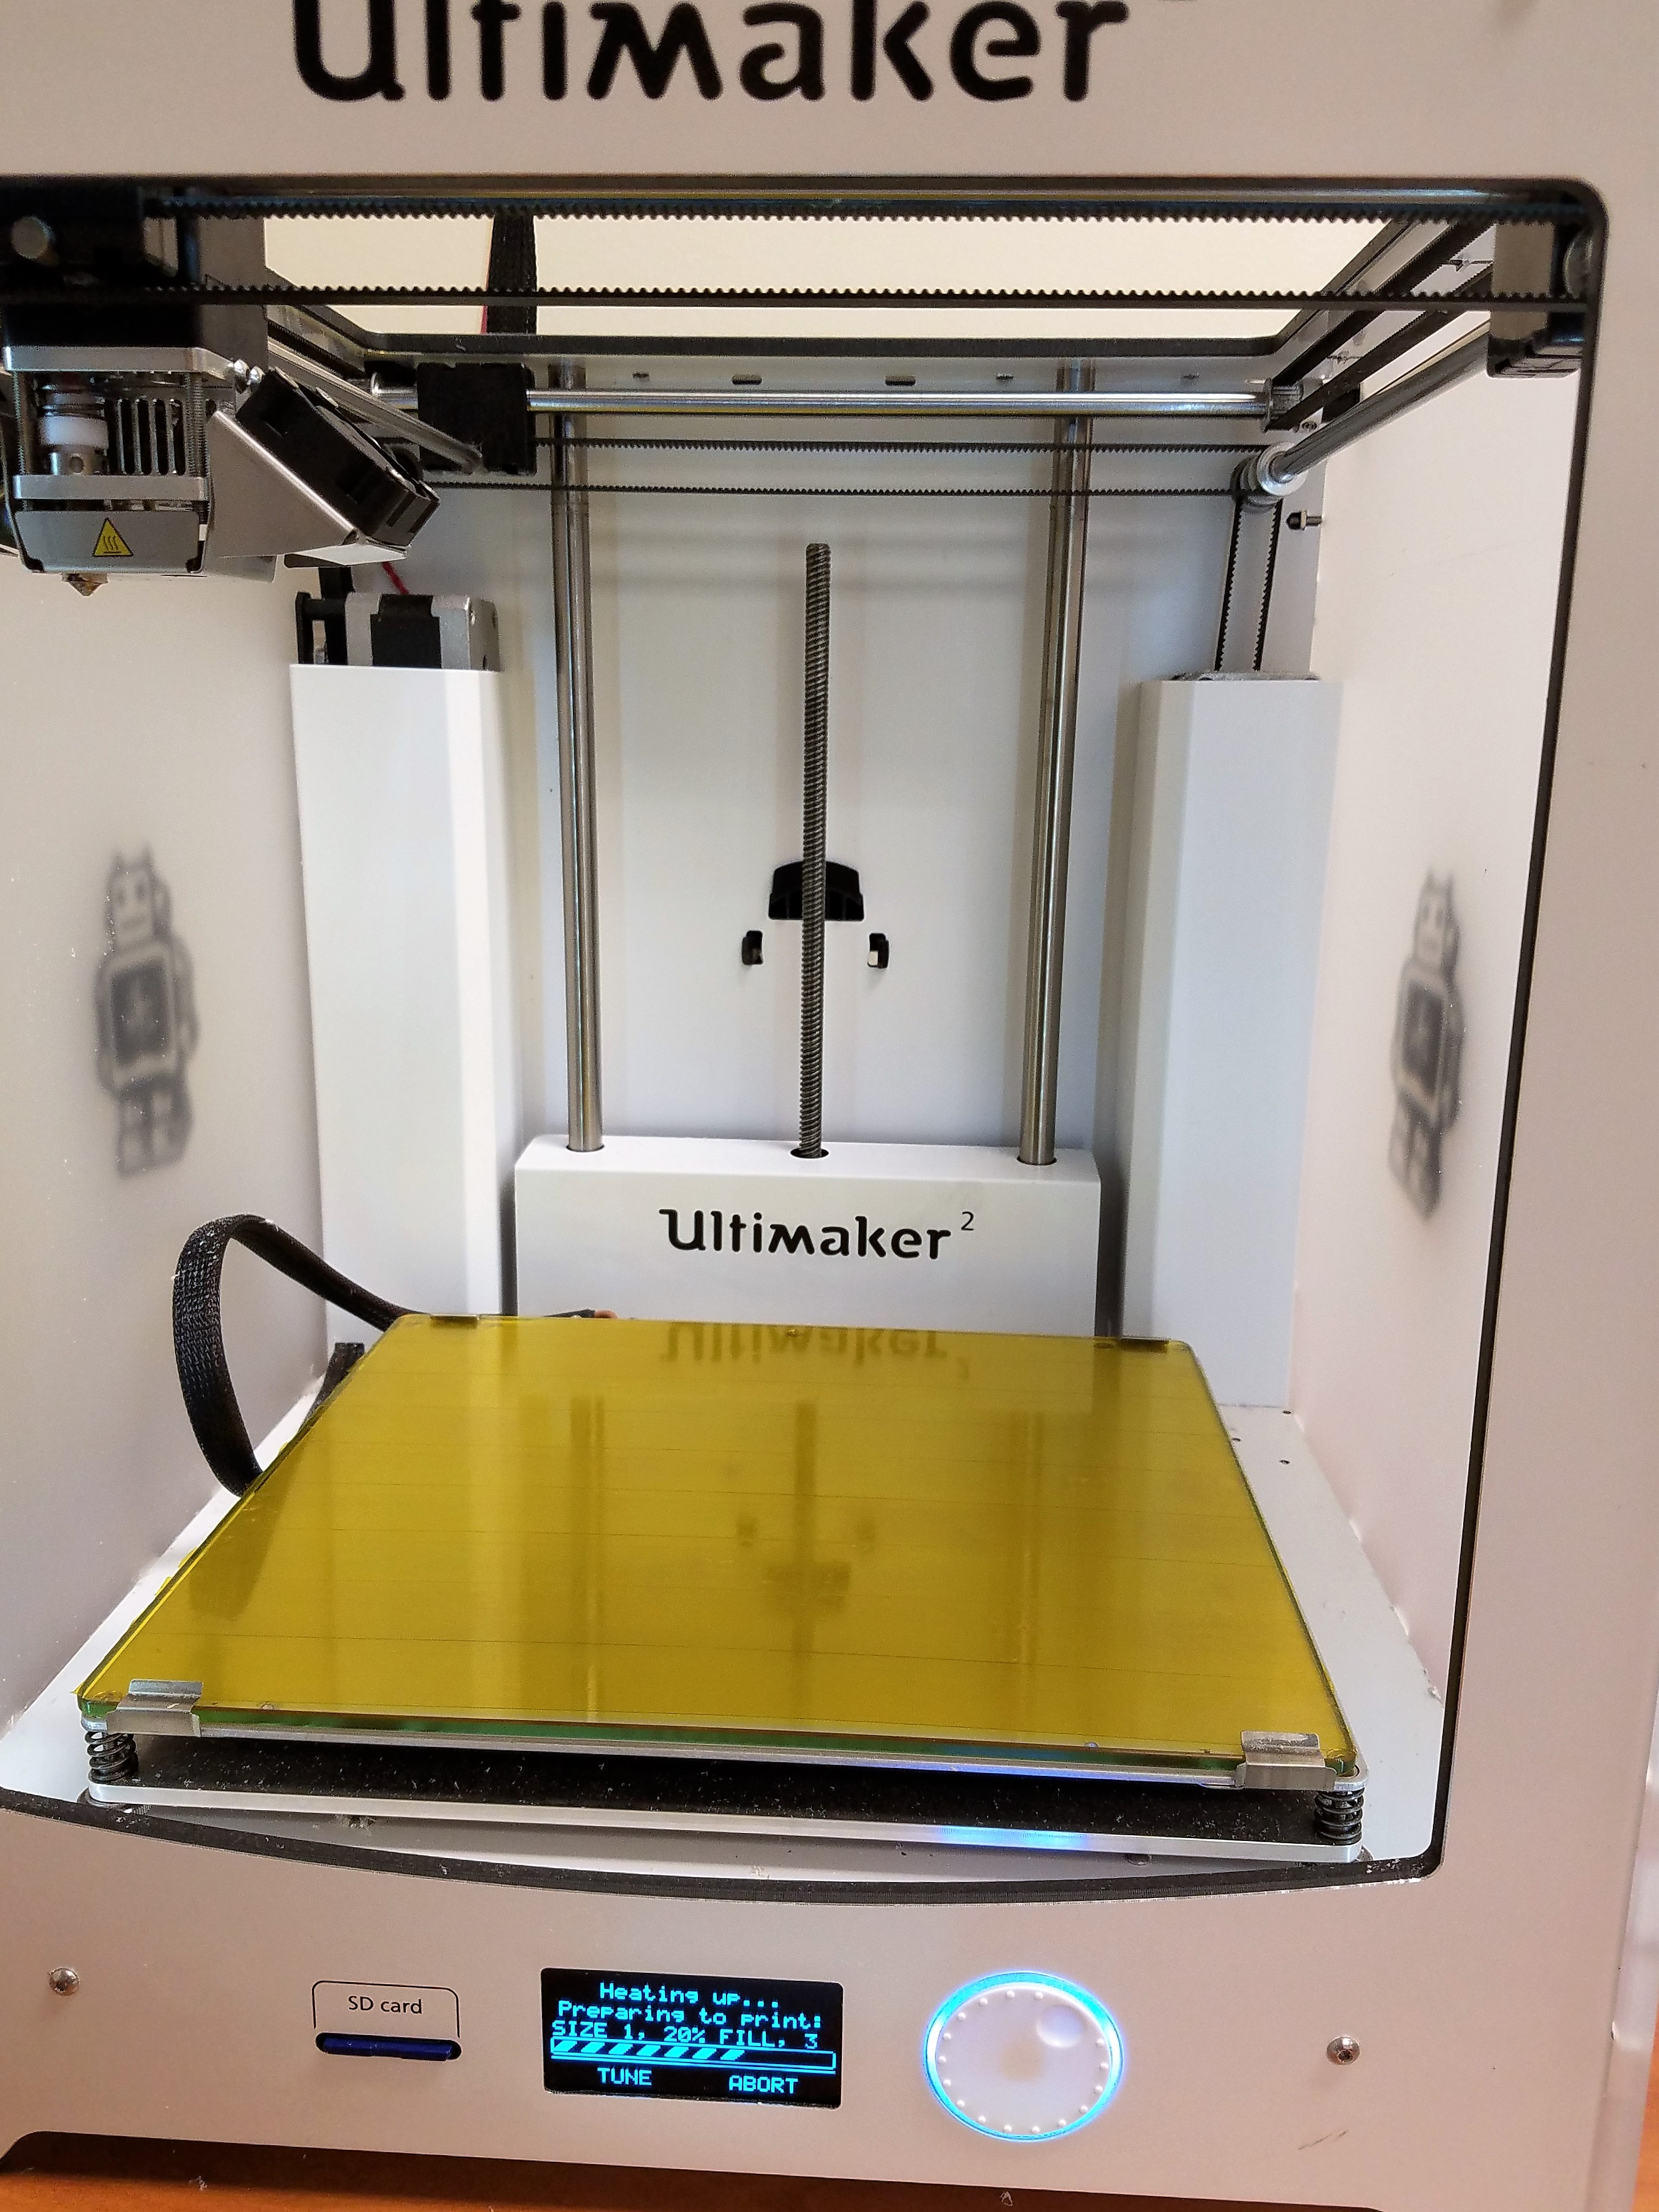
\includegraphics[width=.5\textwidth]{Printer_Clean}
		\label{fig:Printer_Clean}
	\end{figure}
	
\section{Impacts of Research}
	The outcome of the research could provide industries with a significantly cheaper alternative to creating prototypes with expensive metals such as aluminum in order to run real-world tests and showcase their products. Using 3-D printed plastics also creates less waste due to the fact that additive manufacturing methods only require the amount of material needed to create the object, while machining methods could force one to purchase significantly more material than necessary in order to create a part, also contributing to savings. Another benefit to using rapid prototyping is the ability to fairly easily create complex structures that may require expensive outsourcing or costly development methods in order to create a prototype out of a machined metal. Furthermore, using ABS or PLA plastics can be more sustainable due to the fact that the plastics can be recycled into filament for 3-D printing, presumably cheaper than metals.
	
\section{Methods Evaluated}
		The following table outlines the varied fabrication methods used to determine an optimal tensile test specimen for extruded plastics in comparison to metal test specimens. Full detail on specimens and tests will be covered in Chapter 4. Testing was done in three phases with three different purposes:
	\begin{table} [h]
		\centering
		\begin{tabular}{ l l l }
		\noalign{\hrule height 2pt}
		Phase I & Phase 2 & Phase 3 \\ \hline
		Determine Elastic Moduli & Predict Behaviour \& & Determine UTS \\ 
		of ABS \& PLA &Study Print Orientation & of Tensile Specimens\\ \hline
		\end{tabular}
		\caption{Test Phases}
		\label{tab:TestPhases}
	\end{table}
	
	Phase I consisted of designing three sizes of square and rectangular beams such that the beams of each respective size had an identical cross-sectional area. To help rule out fabrication anomalies, three copies of each beam were printed using PLA plastic. The 9 specimens were then tested in a custom-built bending stress test fixture. Data was collected using PASCO electronic sensors and was used to determine an elastic modulus for the specimens. The 9 specimens were also printed with three different in-fill densities in order to determine the effects of density on the strength of the beams. Next, the entire fabrication and testing was repeated using ABS plastic.\par
	In Phase II, predictions were made from the average modulus of elasticity found in Phase I. To do this, I-beams were printed in three different print orientations with three samples each and the top flange, bottom flange, and web were measured. Using these measurements, the Moment of Inertia of each beam was calculated and used along with the average modulus to determine the estimated deflection of the beam when a 40N force was applied. Once this was completed, the beams were tested using the bending stress test fixture used in Phase I. The logged data was compared to the predicted strengths of the beams to determine the accuracy of one's ability to predict structural behavior. Finally, the average modulus of the beams were calculated and compared to the modulus of elasticity of PLA in order to determine the effects of layer orientation on the strength of an object.\par	
	Phase III was intended to be performed by printing out ASME standard conforming plastic tensile test specimens using 100\% in-fill density, along with varying print orientations in the same manner as the I-beams. The specimens would have been tested using a specially designed grip extension for the tensile test machine, as one of the limiting factors of 3D printing is the maximum fabrication size. This data would have been compared to the tensile test results of $\frac{1}{8}$ inch thick sheets of aluminum cut out to according to ASTM standards in order to determine if there was a possible print orientation that behaves comparably to a linear, homogeneous, isotropic material.
	
\section{Terminology Used in this Thesis}
	As a preface to understanding the terminology that will be used throughout this study. Figure \ref{fig:Fill_definition} illustrates what is meant by fill density. The solid hatched border of the squares represents the wall thickness, which is discussed later but is important to note. Figure \ref{fig:Layer_definitiion} defines what is meant when layer orientation is mentioned. For all tensile test studies, the terms Longitudinal and Transverse are used knowing that the force is applied to the face shown by the square cross section in figure \ref{fig:Layer_definitiion}.


	\begin{figure} [H]
		\centering
		\caption{3D Printer Fill Density }
		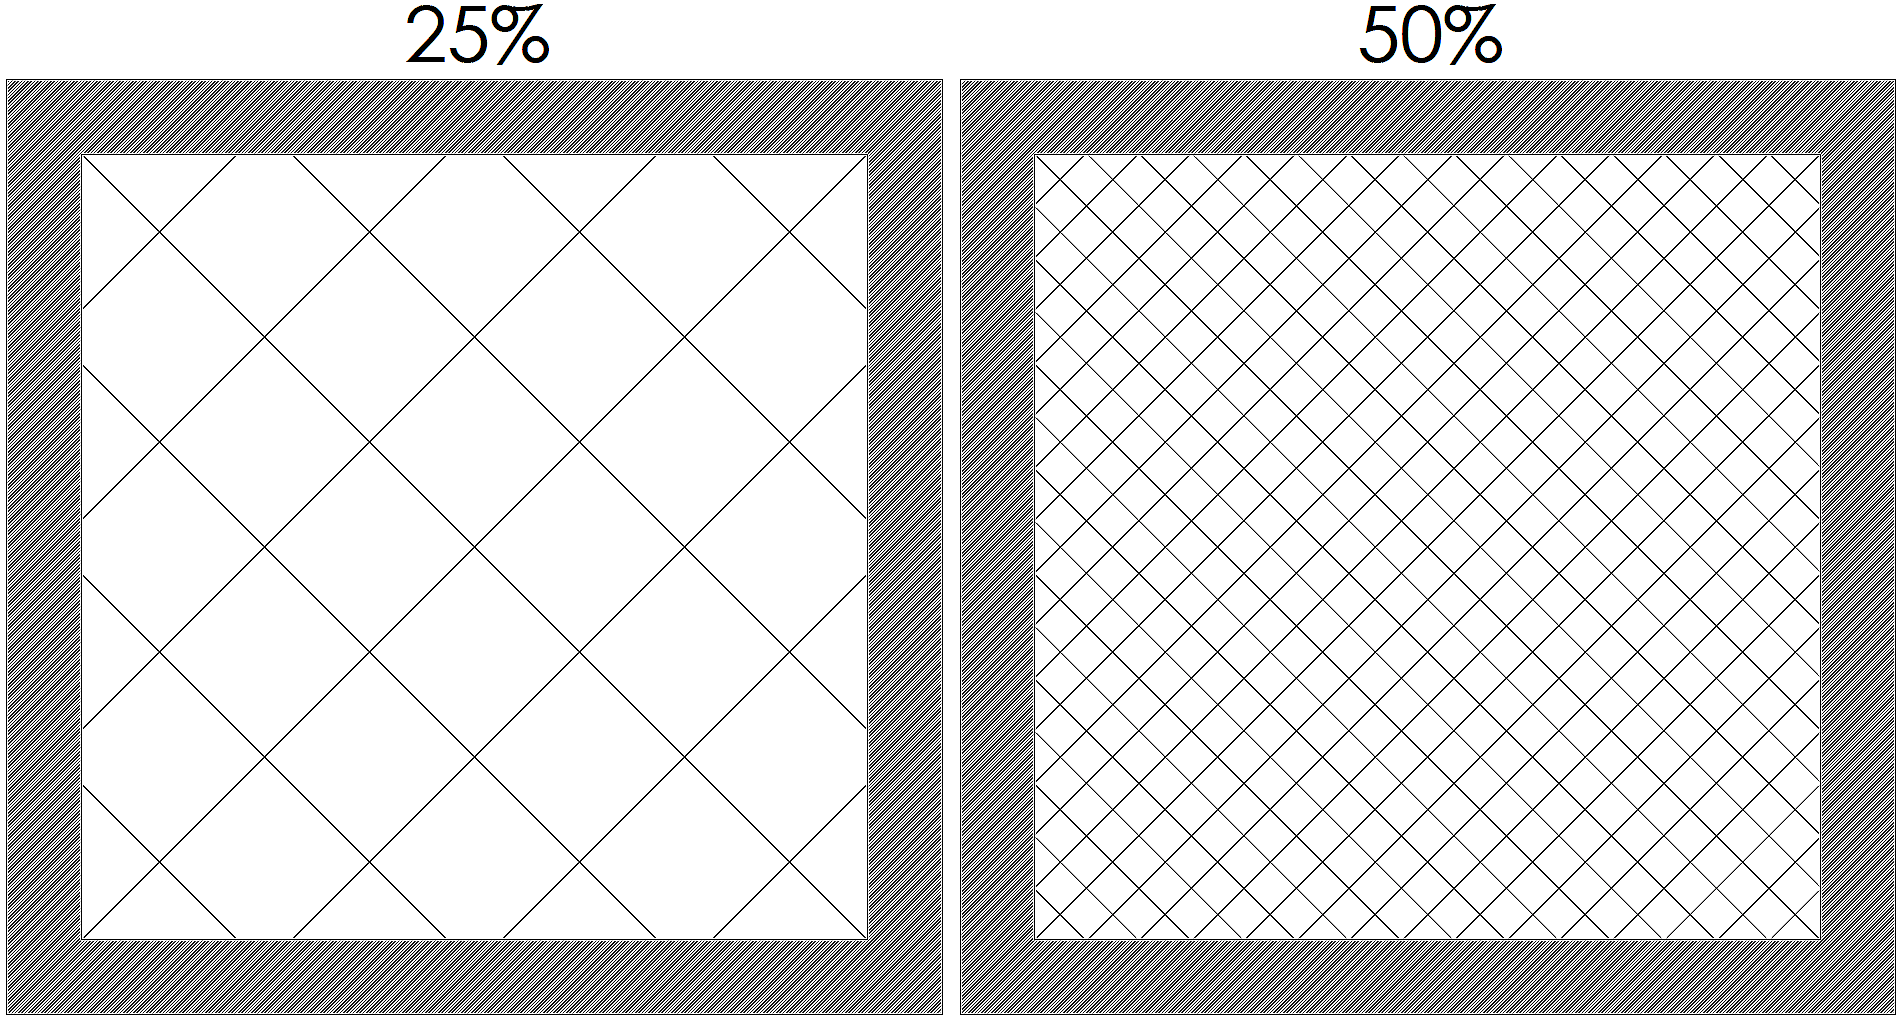
\includegraphics[width=\textwidth]{Definition_Fill}
		\label{fig:Fill_definition}
	\end{figure}
	\begin{figure} [H]
		\centering
		\caption{Print Layer Orientation}
		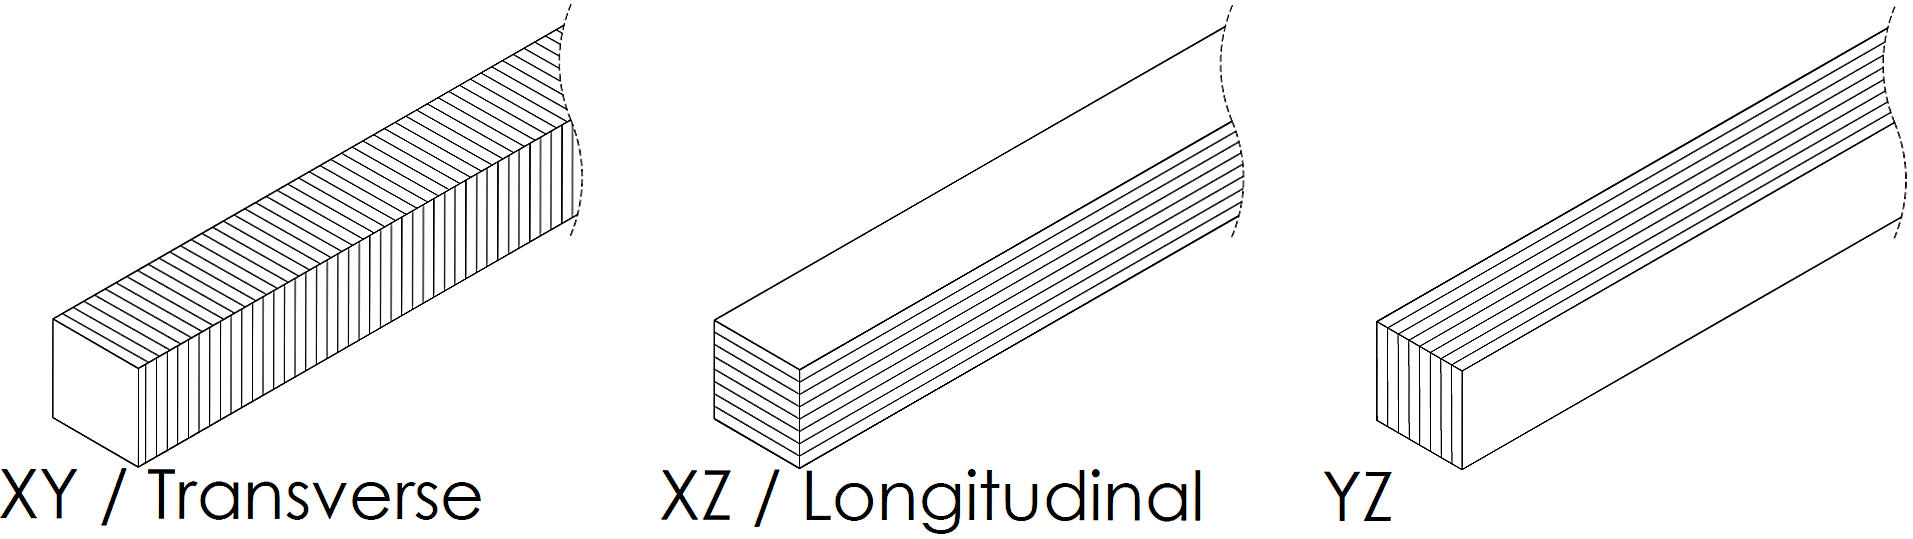
\includegraphics[width=\textwidth]{Definition_Layers}
		\label{fig:Layer_definitiion}
	\end{figure}